% Copyright (c) 2024, Francisco Fernandez
% License: CC BY-SA 4.0
%   https://github.com/fernandezfran/thesis/blob/main/LICENSE
\subsection{Energías de formación}

La ecuación \ref{eq:formacion} de energía de formación definida en la 
sección \ref{ss:electrochim} se presenta usualmente (como en el Materials 
Project \cite{materials_project}) en función de la fracción molar de Si 
($\Theta$ en Li$_{1-\Theta}$Si$_\Theta$), donde su relación con $x$ viene
dada por
\begin{equation}
	x = \frac{1 - \Theta}{\Theta}.
\end{equation}
Los valores de DFT que se utilizan para ajustar ambos conjuntos de parámetros
A y B se presentan en la Figura \ref{fig:eform}a con puntos negros. En azul
y verde se muestran los resultados para los dos conjuntos de parámetros A y B, respectivamente, 
luego de la optimización de pesos. Además, para comparar, se incluyen resultados
obtenidos con la parametrización del ReaxFF realizada por Fan \textit{et al.}
\cite{fan2013}, que es el potencial reactivo del estado-del-arte para este sistema. 
Se observa una buena concordancia para ambos conjuntos de parámetros
de DFTB, en particular el conjunto B resulta ser la mejor de todas las
aproximaciones. Las mayores diferencias entre los modelos DFTB y DFT son para las
aleaciones Li$_{13}$Si$_4$ ($\Theta \approx 0.24$) y Li$_{15}$Si$_4$
($\Theta \approx 0.21$), en especial para esta última. Llamativamente, esta es
la única estructura que obtiene pesos relativos bajos luego del proceso de
\begin{figure}[h!]
	\centering
	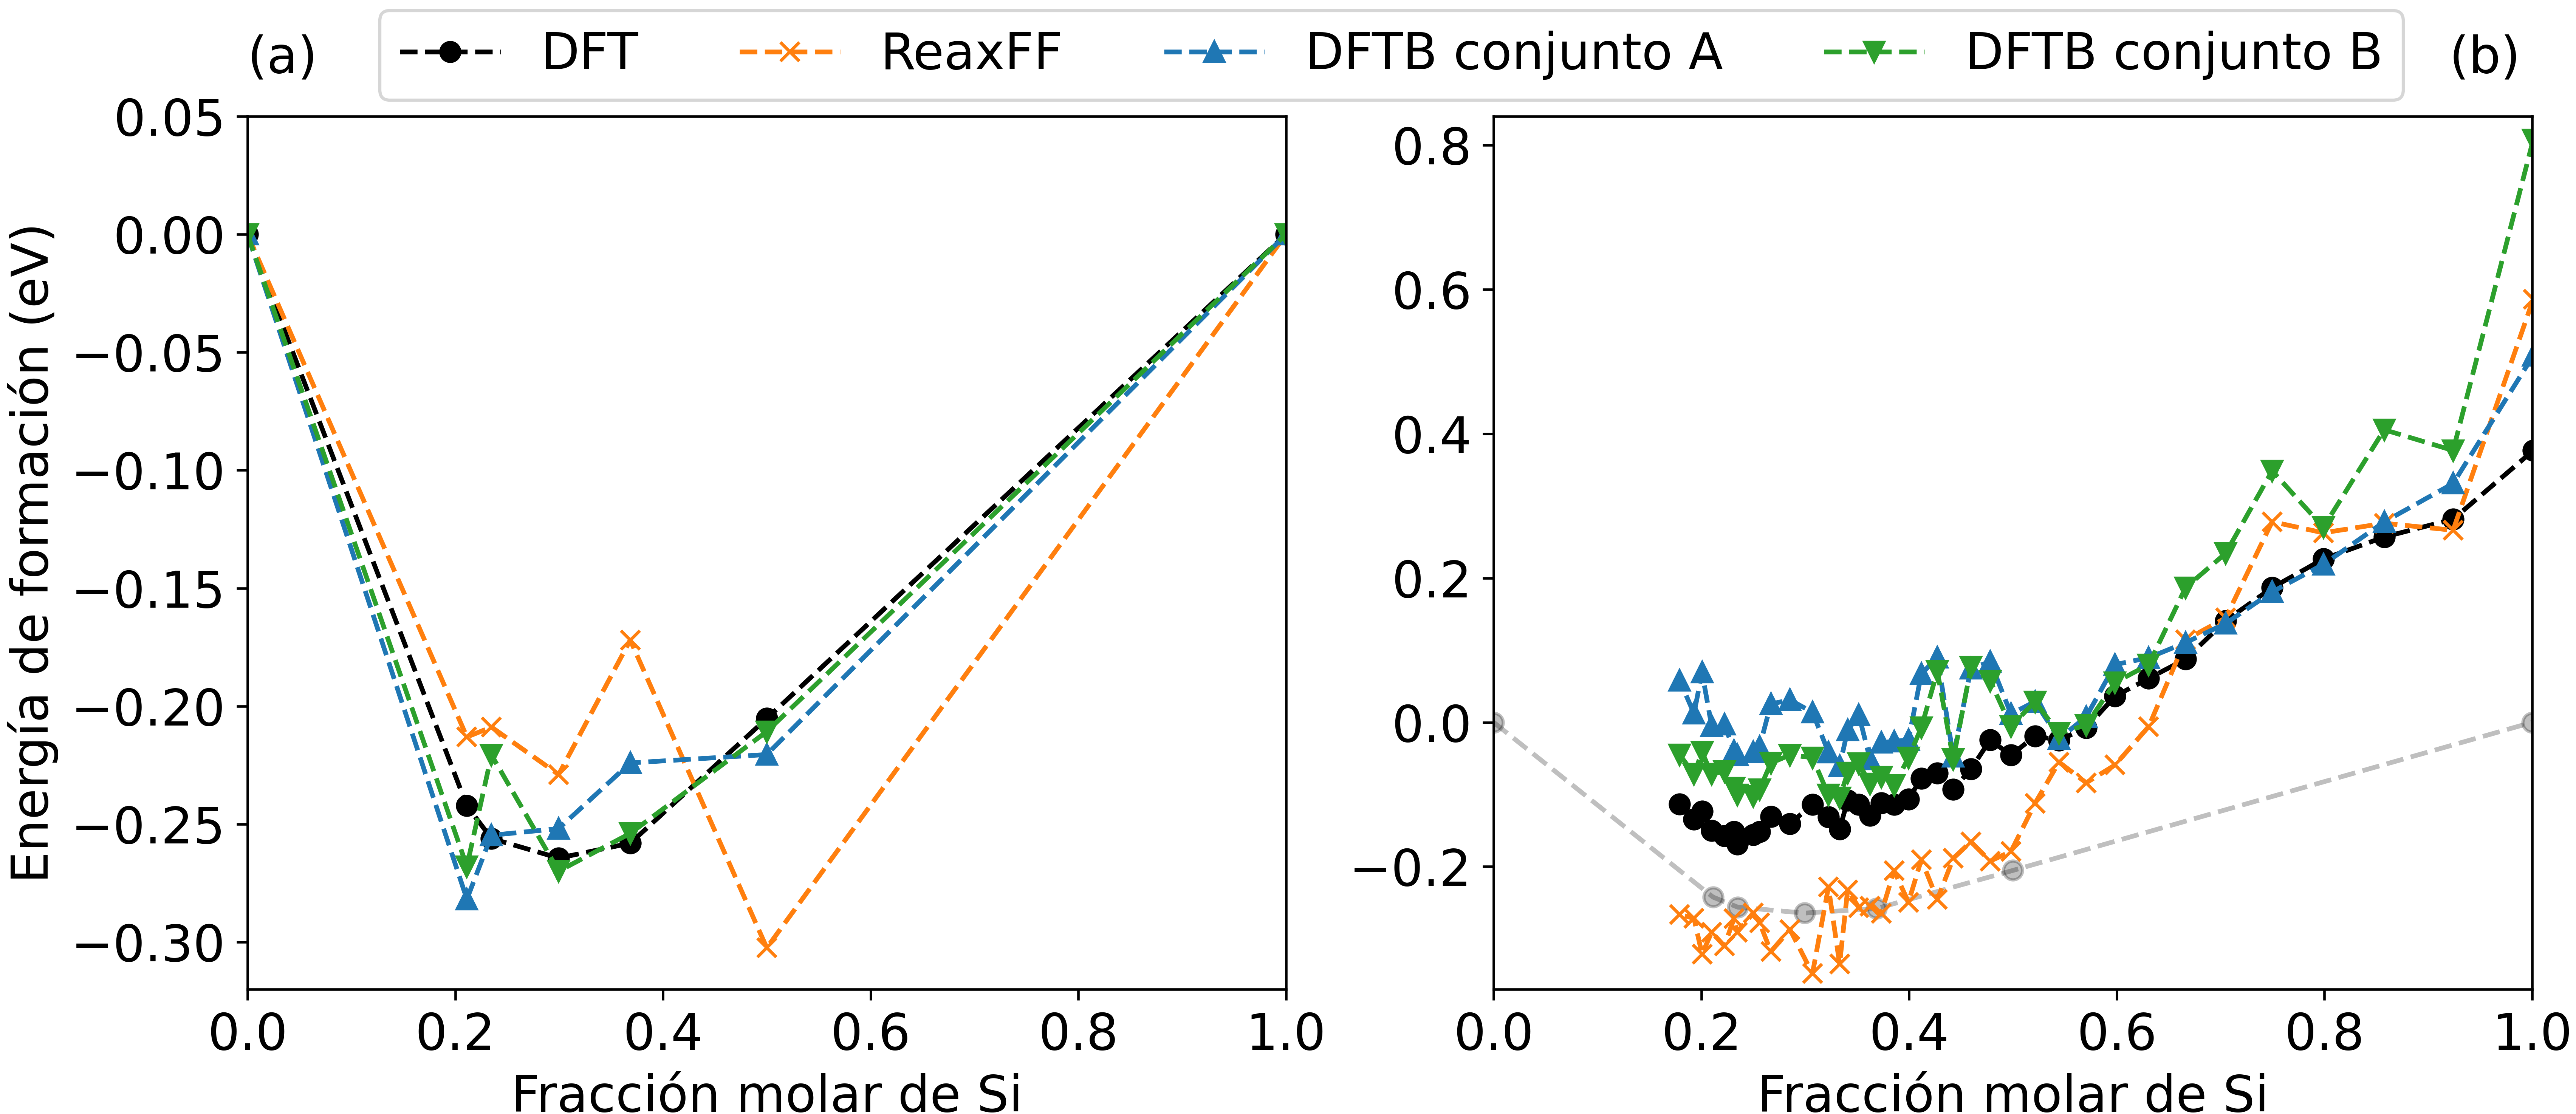
\includegraphics[width=\textwidth]{Silicio/modelo/resultados/formacion/energias.png}
	\caption{Energías de formación calculadas con DFT, ReaxFF y con los dos
	conjuntos A y B de parámetros de este capítulo. (a) Estructuras cristalinas
	de Li-Si de entrenamiento. (b) Estructuras amorfas de Li$_x$Si de evaluación.}
	\label{fig:eform}
\end{figure}
ajuste. Como se mencionó con anterioridad, esto puede indicar que la estructura
de Li$_{15}$Si$_4$ tenga alguna peculiaridad que la haga difícil de ajustar
junto a las otras estructuras del conjunto de datos de entrenamiento. Sin
embargo, hay una mejora general con respecto al potencial ReaxFF para este
sistema y las diferencias obtenidas en las energías de formación son menores.

A continuación se analiza la capacidad de predicción de ambas parametrizaciones
de DFTB para el conjunto de evaluación de estructuras amorfas de Li$_x$Si. Al
igual que para las estructuras cristalinas, se compara con los valores
calculados con DFT y con ReaxFF. La obtención de estas estructuras se introdujo
en la sección \ref{s:dftcalc} y los resultados de las mismas se muestran
en la Figura \ref{fig:eform}b; se deja el caso de los resultados con DFT de
las estructuras cristalinas como referencia. En general, se tiene una buena
reproducción de los valores de DFT con ambas parametrizaciones. Es más, una
inspección minuciosa permite concluir que DFTB es capaz de imitar la tendencia
de los datos DFT, siguiendo la ocurrencia de los distintos máximos y mínimos
locales. Por otro lado, las energías de formación obtenidas con ReaxFF muestran
una desviación considerable con respecto a DFT cuando el silicio se encuentra
mayormente litiado ($\Theta < 0.5$), donde se predice erróneamente que las
estructuras amorfas son incluso más estables que las cristalinas. Otra
observación interesante a resaltar es que las predicciones del conjunto A de
DFTB son significativamente mejores para aleaciones con baja concentración de
litio, mientras que para el conjunto B se cumple lo contrario. La mayor
precisión para cada conjunto se produce para aquellas aleaciones con
concentraciones similares a las estructuras utilizadas para ajustar el término
de energía de banda que son Li$_7$Si$_3$ ($\Theta \approx 0.3$) para el conjunto
B y Li y Si puros para el conjunto A.
